\documentclass[letterpaper,12pt]{article}

\usepackage[utf8]{inputenc}
\usepackage[T1]{fontenc}
\usepackage{lmodern}
\usepackage[french,english]{babel}
\usepackage[margin=1in]{geometry}
\usepackage{amsmath,amssymb,bm}
\usepackage{array,booktabs,longtable}
\usepackage[dvipsnames]{xcolor}
\usepackage{enumitem}
\usepackage{graphicx}
\usepackage{siunitx}
\usepackage[most]{tcolorbox}
% Section, table and page numbers of the thesis come from Document.aux, so they always
% match the final version. Build the thesis first (make), then this file.
\usepackage{xr-hyper}
\usepackage[hidelinks]{hyperref}
\externaldocument[T-]{Document}

\graphicspath{{./images/}}
\setlength{\parskip}{0.5em}
\setlength{\parindent}{0pt}

% The thesis notation (defs.tex) and its acronyms, spelled out here.
% text abbrevs
\newcommand{\eg}{{\it e.g.}}
\newcommand{\ie}{{\it i.e.}}
\newcommand{\etc}{{\it etc.}}

\newcommand{\BEQ}{\begin{equation}}
\newcommand{\EEQ}{\end{equation}}
\newcommand{\BEAS}{\begin{eqnarray*}}
\newcommand{\EEAS}{\end{eqnarray*}}
% std math stuff
% Notation scheme (advisor, 2026-07-30): number sets in \mathbb, general sets in \mathcal,
% vectors lowercase \mathbf, matrices uppercase \mathbf, Greek vectors in \bm.
\newcommand{\ones}{\mathbf 1}
\newcommand{\zeros}{\mathbf 0}
\newcommand{\reals}{\mathbb{R}}
\newcommand{\integers}{\mathbb{Z}}
\newcommand{\eqbydef}{\mathrel{\stackrel{\Delta}{=}}}
\newcommand{\complex}{\mathbb{C}}
\newcommand{\symm}{\mathbb{S}}  % symmetric matrices
\newcommand{\mvec}[1]{\mathbf{#1}}   % vectors (latin): \mvec{x}
\newcommand{\mmat}[1]{\mathbf{#1}}   % matrices: \mmat{A}
\newcommand{\gvec}[1]{\bm{#1}}       % vectors (greek): \gvec{\theta}
\newcommand{\cone}[1]{\mathcal{#1}}  % cones and general sets: \cone{K}
\newcommand{\sign}{{\mbox{\bf sign}}}
\newcommand{\sinc}{{\mbox{\bf sinc}}} 

\newcommand{\Div}{\nabla \!\cdot\!}

% lin alg stuff
\newcommand{\Span}{\mbox{\textrm{span}}}
\newcommand{\Range}{\mbox{\textrm{range}}}
\newcommand{\nullspace}{{\mathcal N}}
\newcommand{\range}{{\mathcal R}}
\newcommand{\Nullspace}{\mbox{\textrm{nullspace}}}
\newcommand{\Rank}{\mathop{\bf Rank}}
\newcommand{\Tr}{\mathop{\bf Tr}}
\newcommand{\diag}{\mathop{\mathrm{diag}}}
\newcommand{\lambdamax}{{\lambda_{\rm max}}}
\newcommand{\lambdamin}{\lambda_{\rm min}}
%XXX dumb question: do we not use \diag(...) to form diagonal or
%block diagonal matrices?

% probability stuff
\newcommand{\Expect}{\mathop{\bf E{}}}
\newcommand{\expect}[1]{\mathop{\bf E{}}[#1]}
\newcommand{\Prob}{\mathop{\bf Prob}}
\newcommand{\erf}{\mathop{\bf erf}}

% convexity & optimization stuff
\newcommand{\Co}{{\mathop {\bf Co}}}
\newcommand{\co}{{\mathop {\bf Co}}}
% \newcommand{\Var}{\mathop{\bf var{}}}
\newcommand{\dist}{\mathop{\bf dist{}}}
\newcommand{\Ltwo}{{\bf L}_2}
%\newcommand{\QED}{~~\rule[-1pt]{8pt}{8pt}}\def\qed{\QED}
\newcommand{\approxleq}{\mathrel{\smash{\makebox[0pt][l]{\raisebox{-3.4pt}{\small$\sim$}}}{\raisebox{1.1pt}{$<$}}}}
\newcommand{\argmin}{\mathop{\rm argmin}}
\newcommand{\epi}{\mathop{\bf epi}}
\newcommand{\hypo}{\mathop{\bf hypo}}
\newcommand{\var}{\mathop{\bf var}}
\newcommand{\avg}{\mathop{\bf avg}}

\newcommand{\vol}{\mathop{\bf vol}}
\newcommand{\Vol}{\mathop{\bf vol}}
\newcommand{\Card}{\mathop{\bf card}}

\newcommand{\dom}{\mathop{\bf dom}}
\newcommand{\aff}{\mathop{\bf aff}}
\newcommand{\cl}{\mathop{\bf cl}}
\newcommand{\Angle}{\mathop{\bf angle}}
\newcommand{\intr}{\mathop{\bf int}}
\newcommand{\relint}{\mathop{\bf rel int}}
\newcommand{\bd}{\mathop{\bf bd}}
\newcommand{\vect}{\mathop{\mathrm{vec}}}
\newcommand{\dsp}{\displaystyle}
\newcommand{\foequal}{\simeq}
\newcommand{\VOL}{{\mbox{\bf vol}}}
\newcommand{\argmax}{\mathop{\rm argmax}}
\newcommand{\xopt}{x^{\rm opt}}

\newcommand{\prox}{\mathbf{prox}}

\newcommand{\SURE}{\textrm{SURE}}
\newcommand{\SURECR}{\textrm{SURE-CR}}

\usepackage{relsize} % Relsize package needed
\usepackage{bm} % Bold greek for parameter vectors (\gvec)

\newcommand{\hutchpp}{\text{Hutch\raisebox{0.35ex}{\relscale{0.75}++}}}

%% new commands from CVXPY paper
\newcommand\plotzero{{\color{gray}0}}
\newcommand\annotatedop[2]{\phantom{\ensuremath{#2}}\hspace{2ex}\ensuremath{#1}\hspace{2ex}{\color{gray}\ensuremath{#2}}}

\newcommand{\ac}[1]{#1}

% A thesis reference: \tref{label} gives "§4.2, p. 61" from the thesis.
\newcommand{\tsec}[1]{\S\ref{T-#1}}
\newcommand{\tpage}[1]{p.~\pageref{T-#1}}
\newcommand{\tref}[1]{\tsec{#1}, \tpage{#1}}

% A committee question, our response, and the new text of the thesis, quoted.
\newcommand{\question}[2]{\par\bigskip\textbf{Q#1.} \emph{#2}\par}
\newtcolorbox{thesisquote}[1]{breakable, enhanced, colback=NavyBlue!4, colframe=NavyBlue!60,
  boxrule=0.4pt, arc=1pt, left=6pt, right=6pt, top=4pt, bottom=4pt, fontupper=\small,
  title={\small Changes in the thesis, #1}, coltitle=black, colbacktitle=NavyBlue!12}

\begin{document}

\begin{center}
{\Large\bfseries Response to the committee}\\[0.5em]
\emph{A Lightweight Canonicalization Engine in C for Disciplined Convex Programming}\\[0.3em]
William Zijie Zhang (2362162), Master's thesis, Electrical Engineering, Polytechnique
Montréal\\
Supervisor: Antoine Lesage-Landry\\[0.3em]
\today
\end{center}

\noindent To Sébastien Le Digabel (chair), Antoine Legrain (second member) and Antoine
Lesage-Landry (supervisor).

\begin{otherlanguage}{french}
\section*{Message au jury}

Bonjour chers membres du jury,

Je voulais tout d'abord vous remercier pour vos commentaires sur mon mémoire. Comme vous m'avez
demandé de clarifier et d'approfondir plusieurs points des résultats, j'ai pris le temps de les
rendre plus complets, et j'ai aussi découvert quelques erreurs dans les affirmations que j'avais
faites sur les contributions.

Premièrement, il y a maintenant quatre problèmes qui sont plus lents. J'ai ajouté une section du
mémoire pour les décrire (\tsec{sec:bench-slower}). Trois des quatre problèmes peuvent devenir
plus rapides. Deux d'entre eux le deviennent avec des changements dans le «~frontend~» (par
frontend, je fais référence à la manipulation des arbres d'expression avant le calcul des
dérivées). Par exemple, pouvoir détecter que \texttt{D @ ones} (où \texttt{D} est une matrice
quelconque) équivaut à \texttt{D.sum(axis=1)}, la somme sur les colonnes, est un grand avantage.
Le troisième, ConvexPlasticity, le devient avec un test de densité. Ces changements ne règlent
pas tout : une partie du ralentissement vient du moteur lui-même, en particulier de la mémoire
de la disposition globale (Q5).

Deuxièmement, j'ai refait toutes les mesures sur un ordinateur plus récent (MacBook M2 de 2022,
avec Apple \texttt{Accelerate}), plutôt que sur l'ordinateur Intel de 2018 de la version
soumise, pour que les résultats soient reproductibles sur du matériel actuel, comme celui de la
plupart des utilisateurs de \texttt{CVXPY}. Pour la première canonicalisation, les ratios et les
temps sont semblables. Pour les re-résolutions paramétriques, en revanche, \texttt{diffengine}
n'est plus plus rapide que sur deux des sept problèmes. Les nouvelles mesures par phase
expliquent où va le temps : la passe numérique ne prend que $3$ à $20\,\%$ d'une re-résolution,
et le reste sert à convertir les matrices au format CSC et dans l'ordre des cônes du solveur,
alors que le tenseur de \texttt{CVXPY} produit directement ce format. J'ai donc modifié les
affirmations de ma conclusion et de la discussion des résultats pour dire seulement qu'il y a
des bénéfices, mais que la séparation ne remplace pas encore le tenseur pour les re-résolutions.
% TODO(William): the version sent to the jury had faster re-solves on more problems. Confirm
% whether the change comes from the machine, from the engine/CVXPY versions, or both.

Troisièmement, le problème UnconstrainedQP n'était pas réellement 100 fois plus rapide. C'était
dû à un changement de frontend que j'avais appliqué sur la branche du backend
\texttt{diffengine}, mais pas sur celles des autres. En l'appliquant à tous, cet avantage
disparaît. Ceci a été rectifié : aucun backend n'utilise maintenant ce changement.

À part ces trois points, qui sont les changements majeurs, j'ai aussi fait les études
d'ablation et exécuté plus d'instances de benchmark, avec des mesures de signification
statistique, ce qui répond à tous vos commentaires.

J'ai rédigé moi-même les réponses à vos questions. Claude, l'outil d'IA déclaré dans le
mémoire, les a ensuite reformulées et mises en forme en anglais ; les chiffres viennent
directement des scripts de mesure.
\end{otherlanguage}

\section{Summary of corrections}

I have made all the modifications required by the committee and by Antoine Legrain's
examiner report, as well as the minor corrections that Sébastien Le Digabel annotated and those
listed in the appendix of Antoine Legrain's report. The minor corrections are not listed here.
All changes since the version sent to the committee are marked in \texttt{Document-diff.pdf},
with added text in blue and deleted text in red. Section, table and page numbers below refer to
the final version.

Table~\ref{tab:required} lists the required modifications. ``J'' refers to the committee's
requirements after the defence, and (i)--(vii) to the items of the synthesis of the examiner
report. Each item is answered in detail, with the new results, in
Sections~\ref{sec:replies} and~\ref{sec:results}.

{\small
\begin{longtable}{>{\raggedright}p{0.17\textwidth} >{\raggedright}p{0.50\textwidth}
  >{\raggedright\arraybackslash}p{0.25\textwidth}}
\caption{Required modifications and where they are made.}\label{tab:required}\\
\toprule
Request & Change & Where \\
\midrule
\endfirsthead
\toprule
Request & Change & Where \\
\midrule
\endhead
\bottomrule
\endfoot
J1a: statistical significance
  & Every timed comparison is made in $30$ runs and tested per problem with a two-sided
    Mann--Whitney $U$ test~\cite{mann1947}, Holm-adjusted~\cite{holm1979} over the problems,
    and over the suite with a Wilcoxon signed-rank test~\cite{wilcoxon1945} and a bootstrap
    confidence interval. Significant ratios are starred in the tables and filled in the
    figures (Section~\ref{sec:results}).
  & Ch.~4 introduction, \tpage{sec:Theme2}; \tsec{sec:bench-oneshot} \\
J1b, (ii): ablation
  & The dense blocks are turned off on all $25$ problems, for time and memory, and on the
    re-solves together with the split (Section~\ref{sec:res-ablation}).
  & \tref{sec:bench-ablation} \\
J1c: more instances
  & Each run draws new parameter values from its own seed, and every problem is also scaled
    in size and density (J1d).
  & Ch.~4 introduction; \tsec{sec:bench-sensitivity} \\
J1d: sensitivity to size and sparsity
  & All $25$ problems at five sizes, $s \in \{1/4, 1/2, 1, 2, 4\}$, and eight problems at seven
    densities, with and without the dense blocks (Section~\ref{sec:res-sensitivity}).
  & \tref{sec:bench-sensitivity} \\
J1e, (iii): non-DPP problems
  & Re-solves of two families in DPP, non-DPP and parameter-free variants, and of
    ConvexPlasticity, the suite's one non-DPP parametric problem (Q3).
  & \tref{sec:bench-nondpp} \\
J2, (i): related literature and DNLP
  & Matrix-free modelling, \texttt{CVXcanon}, \texttt{CVXGEN}, \texttt{Convex.jl}~0.16,
    \texttt{Pyomo}'s persistent interfaces, block-sparse antecedents (finite elements,
    \texttt{Ceres}, \texttt{g2o}), and sparse factorization as the origin of the
    symbolic/numeric split. The thesis now states who leads \texttt{SparseDiffEngine} and what
    is specific to this work (Q6).
  & \S\ref{T-sec:computing-derivatives}, \tsec{sec:contributions},
    \tsec{sec:theme1-atom-classes} \\
J3: declaration of AI use
  & New front-matter page.
  & Front matter \\
(iv): repeated measurements
  & $30$ runs, each in a fresh process; tables give mean $\pm$ standard deviation.
  & Ch.~4 introduction; Table~\ref{T-tab:oneshot-compile} \\
(v): dimensions of the instances
  & $m$, $n$, $\mathrm{nnz}(\mmat{A})$, $\mathrm{nnz}(\mmat{P})$, parameter size and DPP
    status of every problem.
  & Appendix~\ref{T-app:bench}, Tables~\ref{T-tab:instances-desc} and~\ref{T-tab:instances} \\
(vi): time by phase
  & The share of each phase on the four slower problems, their formulations and the
    mechanism for each (Section~\ref{sec:res-slower}).
  & \tref{sec:bench-slower} \\
(vii): correctness check
  & The problem data are checked against the \texttt{CPP} backend to a relative tolerance of
    $10^{-9}$, at the first canonicalization and after a parameter update.
  & Ch.~4 introduction \\
\end{longtable}}

\paragraph{A change of baseline.}
The version sent to the committee reported a $2.8\times$ geometric-mean speedup of
\texttt{diffengine} over the best \texttt{CVXPY} backend. Two things have changed since. First,
all experiments were rerun on an Apple M2 with the current versions of \texttt{CVXPY} and
\texttt{SparseDiffEngine}. Second, the earlier comparison was not fair: \texttt{diffengine} was
timed with \texttt{CVXPY} pull request \#3524, which reassociates chains of matrix products that
end in a constant, while the other backends were timed without it. That pull request speeds up
every backend, so now none of them uses it.
% N30: update the numbers below from results/thesis-n30/facts.json.
With this baseline, \texttt{diffengine} is the fastest of the four backends on $21$ of the $25$
problems, significantly on all $21$, with a geometric-mean ratio of $0.43$ to the best
\texttt{CVXPY} backend, about $2.3\times$ faster. UnconstrainedQP is now $11.8\times$ slower;
Section~\ref{sec:res-slower} explains why.

\section{Replies to the defence questions}\label{sec:replies}

\question{1}{Why materialize dense blocks rather than leave them as operators, as in the
matrix-free approach of Diamond and Boyd~\cite{diamond2016matrixfree}? When is each approach
preferable?}
Because the solvers that \texttt{CVXPY} calls need the matrices. Its default solvers are
\texttt{Clarabel}, an interior-point method, and \texttt{OSQP} and \texttt{SCS}, which are
first-order methods; commercial solvers such as \texttt{MOSEK} and \texttt{Gurobi} are
interior-point or simplex methods. All of them factorize a matrix built from $\mmat{A}$ and
$\mmat{P}$: an interior-point method factorizes a KKT system at every iteration, and
\texttt{OSQP} and \texttt{SCS}, in their default direct mode, factorize their KKT matrix once and
reuse the factorization across iterations. So every one of them needs $\mmat{A}$ and $\mmat{P}$ explicitly,
whatever its algorithm. Matrix-free modelling pays off for very large problems built from fast
transforms, solved by first-order methods that only need products with $\mmat{A}$ and
$\mmat{A}^\top$, such as the indirect mode of \texttt{SCS}. A permuted dense block lies between
the two: it is a materialized matrix, but it keeps the structure of the operator, namely its
row and column selectors and its dense block.

\begin{thesisquote}{\tref{sec:computing-derivatives}}
In convex optimization, Diamond and Boyd take the matrix-free view. Instead of forming
$\mmat{A}$, they represent the problem as a graph of linear operators, available only through
their forward and adjoint products, which suits first-order solvers. The solvers that
\texttt{CVXPY} calls by default instead factorize a matrix built from $\mmat{A}$ and $\mmat{P}$.
The matrix-free approach pays off on very large problems built from fast transforms, such as
convolutions and Fourier transforms, and it needs solvers that accept operators instead of
matrices. The permuted dense matrices of \S3.2 sit between the two: they form the matrix that
the solver factorizes, but keep the structure of the operator, its row and column selectors and
its dense block.
\end{thesisquote}

\question{2}{If the permuted dense representations are disabled, what fraction of the speedup
remains?}
% N30: update the numbers and insert Figure B (the ablation) here.
Most of it. Without the dense blocks, \texttt{diffengine} is $2.17\times$ faster than the best
\texttt{CVXPY} backend in geometric mean, against $2.33\times$ with them. The difference between
the two, $1.07\times$, is not significant over the suite (Wilcoxon signed-rank, $p = 0.07$).
Per problem, the effect is large in both directions, as Figure~\ref{fig:ablation} shows. On six
problems with dense data, the dense blocks take the engine from about $3$ to about $7\times$
faster than \texttt{CVXPY}. On UnconstrainedQP they take it from $4\times$ faster to $11.8\times$
slower, and on ConvexPlasticity from $1.4$ to $6.9\times$ slower, because both build a dense
block from data that is sparse in fact.

The split between the symbolic and the numeric pass plays no part in a first
canonicalization, because each pass runs once. It is ablated on the re-solves instead
(Section~\ref{sec:res-ablation}). The dense blocks are the only part of the engine that can be
turned off on a first canonicalization while keeping everything else the same. The other
differences from \texttt{CVXPY}'s backends, namely the implementation in C, one Jacobian per
node and the global layout, are built into every atom and cannot be switched off one at a time.
We therefore do not attribute the remaining $2.17\times$ to any one of them.

\question{3}{How does re-solving behave on a non-DPP parametric problem?}
% N30: update the numbers.
On the two families written with a product of two parameters, which \ac{DPP} forbids, the cached
re-solve of \texttt{diffengine} is $12\times$ faster than \texttt{CVXPY} on \texttt{lasso} and
$13\times$ on \texttt{factor\_cov}, in both cases over all $30$ runs (Table~\ref{tab:res-nondpp}
gives the means), because \texttt{CVXPY}
has to canonicalize the problem again at every solve.
ConvexPlasticity, the suite's only natural non-DPP parametric problem, is the exception: it
re-solves in $204$~ms against $42$~ms for \texttt{CVXPY}. The split is not the cause: $88\,\%$ of
that re-solve assembles the dense $3000 \times 3000$ block of $\mmat{P}$, built from a diagonal
given as a dense array. Without the dense blocks, the same cached re-solve takes $2.3$~ms,
$18\times$ faster than \texttt{CVXPY}. The split therefore carries over to a real non-DPP
problem; what fails there is the dense storage of a constant that is sparse in fact.

The non-DPP experiment is new in the thesis. The thesis also no longer claims that the split
replaces the tensor: the discussion now says that the split re-solves within a small factor of
the tensor without requiring \ac{DPP}, and much faster than \texttt{CVXPY} when the problem is
not \ac{DPP}.
% N30: quote the final text of sec:bench-nondpp and of the discussion here.

\question{4}{Why not re-evaluate only the subtrees that depend on the updated parameters?}
The engine now does this: after a parameter update, the numeric pass re-evaluates only the
subtrees that contain a parameter, and keeps the cached values of the others. All re-solve
times in the thesis use it. With it, the numeric pass takes $3$ to $20\,\%$ of a re-solve on the
five problems where the tensor is faster. The rest is the conversion of the output to
compressed sparse columns in the cone order of the solver, which is now the first item of
future work.

\begin{thesisquote}{\tref{sec:theme1-problem-interface}}
The numeric pass therefore skips an affine tree after the first evaluation, until the next
parameter update. After an update, it re-evaluates only the subtrees that contain a parameter,
and keeps the cached values of the others.
\end{thesisquote}

\question{5}{When does the global layout become a handicap relative to \texttt{CVXPY}'s local
layout, in particular for memory?}
When the problem has many variables and many nodes. In the global layout, each node keeps,
besides its Jacobian, integer work arrays of length $n$, the total number of variables, whatever
variables its own subtree contains. Their memory is therefore $O(\text{nodes} \times n)$
integers. In \texttt{CVXPY}'s local layout, each node stores blocks only for the variables it
depends on, so the same overhead is proportional to the sum, over the nodes, of the number of
variables each one depends on. The two coincide when every node depends on every variable, and
the local layout wins when most nodes depend on a few variables out of many.

OptimalAdvertising shows it. Each of its $250$ minimum terms depends on one row of a
$250 \times 1000$ variable, but has a Jacobian over all $250\,000$ variables, and the symbolic
pass visits every column. Without the dense blocks, its peak memory is $945$~MB, against $173$ to
$197$~MB for the \texttt{CVXPY} backends; that difference is the per-node cost. With the dense
blocks it reaches $6.1$~GB, and most of the difference comes from the aggregate constraints
$\mmat{D}^\top \ones \le \mvec{t}$ and $\mmat{D} \ones \ge \mvec{c}$. Canonicalized alone,
$\mmat{D}^\top \ones \le \mvec{t}$ takes $4$~GB with the dense blocks and $112$~MB without. Its
Jacobian is stored as $1000$ dense blocks of $250$ entries, but each block also keeps an inverse
map of its columns with one integer per variable of the problem, $250\,000$ of them. This is
the cost of the global layout again, paid once per dense block rather than once per node.
Storing these maps sparsely, or sharing one workspace across the blocks, should remove most of
it.

Both aggregate constraints are sums written as products with a vector of ones. The converter
from \texttt{CVXPY} to the engine can recognize a product $\mmat{D}\ones$ or
$\mmat{D}^\top\ones$ and build the engine's sum atom instead, which builds no dense block. With
this rewrite, OptimalAdvertising canonicalizes in $0.46$~s instead of $1.10$~s, with a peak
memory of $1.4$~GB instead of $6.1$~GB. A weighted sum $\mmat{D}\mvec{w}$ with a general dense
$\mvec{w}$ still needs the fix in the engine.
% N30: rerun the OptimalAdvertising rewrite in the harness at 30 runs (now 3 runs).

\begin{thesisquote}{\tref{sec:Limitations}}
Another part of the memory cost comes from the global layout. Every node of the expression trees
holds a Jacobian over all $n$ variables, together with integer work arrays of length~$n$. The
values stored remain proportional to the nonzeros, but this overhead grows with the number of
nodes times the number of variables. On problems with very many variables and deep trees, it
can exceed the memory of \texttt{CVXPY}'s local layout, whose blocks span only the variables
that each node depends on.
\end{thesisquote}

\question{6}{What part of \texttt{SparseDiffEngine} pre-existed the thesis or was developed for
DNLP, and what part is specific to this work?}
Daniel Cederberg leads \texttt{SparseDiffEngine}. He started it as the differentiation engine
of the \texttt{DNLP} extension of \texttt{CVXPY}~\cite{cederberg2025disciplined}, which
differentiates nonlinear atoms at every iterate of the solver, and I co-developed it with him.
Daniel is from outside our research group, and the version sent to the committee should have
said so clearly; it now does. This thesis uses the engine for a different
purpose, canonicalization: it evaluates the affine atoms and the quadratic form at the origin to
obtain the problem data. What is specific to the thesis is the interface to \texttt{CVXPY},
namely the \texttt{diffengine} backend and its re-solve path for parametric problems, and the
benchmarks of Chapter~4.

\begin{thesisquote}{\tref{sec:contributions}}
\texttt{SparseDiffEngine} is led by Daniel Cederberg, a collaborator from outside our research
group, and the author co-developed it with him. It is the differentiation engine of the
\texttt{DNLP} extension of \texttt{CVXPY}, where it differentiates nonlinear atoms such as
\texttt{exp}, \texttt{log} and \texttt{entr} at every iterate of the solver. This thesis builds
on the observation that canonicalization is a special case of the same computation: once a
problem is canonicalized, only affine atoms and quadratic forms remain, and their derivatives
are the problem data.
\end{thesisquote}
\begin{thesisquote}{\tref{sec:theme1-atom-classes}}
What is specific to this thesis is the interface to \texttt{CVXPY} of \S3.3, namely the
\texttt{diffengine} backend and its re-solve path for parametric problems, and the benchmarks of
Chapter~4.
\end{thesisquote}

\question{7}{What is the strategy for \ac{BLAS} and binary distribution of
\texttt{sparsediffpy}?}
\texttt{cvxcore} is a C++ extension, built with a copy of \texttt{Eigen}, that lives inside the
\texttt{CVXPY} repository, so \texttt{CVXPY} has to compile and ship it.
\texttt{sparsediffpy} is a separate package: \texttt{CVXPY} only declares it as a dependency and
calls it, which keeps the \texttt{CVXPY} side of the backend much simpler. \texttt{sparsediffpy}
is still compiled, in C, and its own wheels are built for Linux, macOS and Windows and published
on \texttt{PyPI}. They link Apple's \texttt{Accelerate} on macOS and bundle \texttt{OpenBLAS} on
Linux and Windows, so users install nothing beyond the package. The thesis did not say this; it
now does, in the section that introduces \texttt{sparsediffpy}.

\begin{thesisquote}{\tref{sec:theme1-api}}
Unlike \texttt{cvxcore}, which is compiled inside the \texttt{CVXPY} repository,
\texttt{sparsediffpy} is a separate package on which \texttt{CVXPY} only depends. Its compiled
wheels for Linux, macOS and Windows link Apple's \texttt{Accelerate} on macOS and a bundled copy
of \texttt{OpenBLAS} on the other two, so users need no \ac{BLAS} of their own.
\end{thesisquote}

\section{The new results}\label{sec:results}
% N30: this whole section is rewritten from results/thesis-n30 once the sweep finishes, with
% Figures A-D and the excerpt tables embedded, and the final thesis text quoted.

\paragraph{Methodology.}
Every timed comparison is made in $30$ runs, each in a fresh process, on an Apple M2 (24~GB,
macOS 26.5.1) with Apple's \texttt{Accelerate}, single-threaded. On each problem, the runs of
\texttt{diffengine} and those of the other backend are compared with a two-sided Mann--Whitney
$U$ test~\cite{mann1947}, Holm-adjusted~\cite{holm1979} over the problems of the comparison. Over
the suite, we test the geometric mean of the ratios with a Wilcoxon signed-rank
test~\cite{wilcoxon1945} on the log-ratios and give its bootstrap $95\,\%$ confidence interval.

The usual rule of at least $30$ observations comes from the normal approximation of a sample
mean. The Mann--Whitney test is a rank test and assumes no normality, so it is valid at $20$
runs as well; with $20$ runs per side, its smallest Holm-adjusted $p$-value over $25$ problems
is already $1.7 \times 10^{-6}$. We nevertheless reran every comparison at $30$ runs, so that
the tables also give stable means and standard deviations.

\subsection{First canonicalization}\label{sec:res-oneshot}
\subsection{Ablation}\label{sec:res-ablation}
\begin{figure}[htbp]
\centering
% 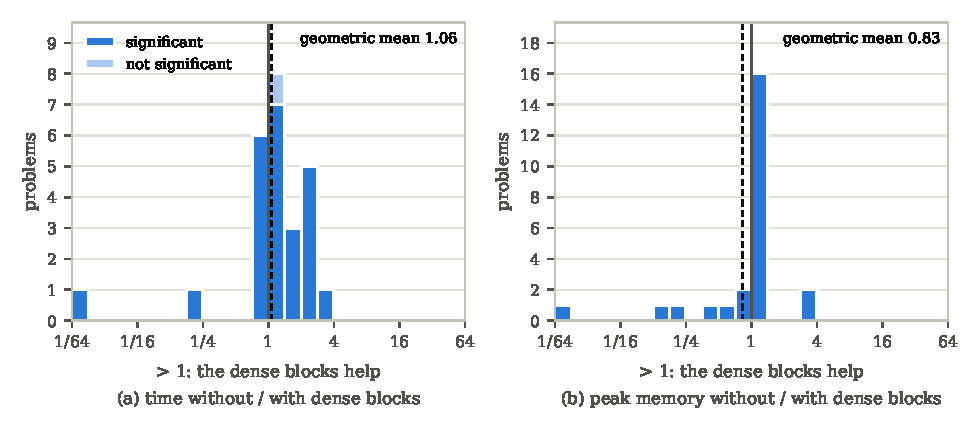
\includegraphics[width=\textwidth]{ablation_thesis}
\caption{Ratio of \texttt{diffengine} to the best \texttt{CVXPY} backend on each problem, with
and without the dense blocks.}\label{fig:ablation}
\end{figure}
\subsection{Sensitivity to size and density}\label{sec:res-sensitivity}
\subsection{The four slower problems}\label{sec:res-slower}
\subsection{Re-solves and non-DPP problems}\label{sec:res-nondpp}
\begin{table}[htbp]
\centering
\caption{Re-solve time on problems that are not DPP.}\label{tab:res-nondpp}
\end{table}

\section{Discussion}\label{sec:discussion}

\bibliographystyle{IEEEtran}
\bibliography{Document}

\end{document}
